\section{Найти и построить область определения сложной функции}
\[
z = \ln{\frac{x^2 + y^2}{x - y}}
\]

\subsection{Условия области определения}

\begin{enumerate}
\item Логарифм определён, когда его аргумент \(> 0\):
\[
\frac{x^2 + y^2}{x - y} > 0
\]

\item Знаменатель не равен нулю:
\[
x - y \neq 0 \quad \Rightarrow \quad x \neq y
\]
\end{enumerate}

\subsection{Анализ знака дроби}

Числитель \(x^2 + y^2 \ge 0\), причём \(x^2 + y^2 = 0\) только при \(x = 0, y = 0\).

Точка \((0,0)\) не входит в ОДЗ, так как дробь \(\frac{0}{0}\) не определена.

Таким образом, числитель \(x^2 + y^2 > 0\) для всех \((x, y) \neq (0,0)\).

Дробь положительна, когда числитель и знаменатель одного знака:
\[
x - y > 0 \quad \Rightarrow \quad x > y
\]

\subsection{Итоговая область определения}
\[
\boxed{D = \{ (x, y) \in \mathbb{R}^2 \mid x > y, \ (x, y) \neq (0,0) \}}
\]

\subsection{Графическое представление}

\begin{figure}[h] % h = here
    \centering
    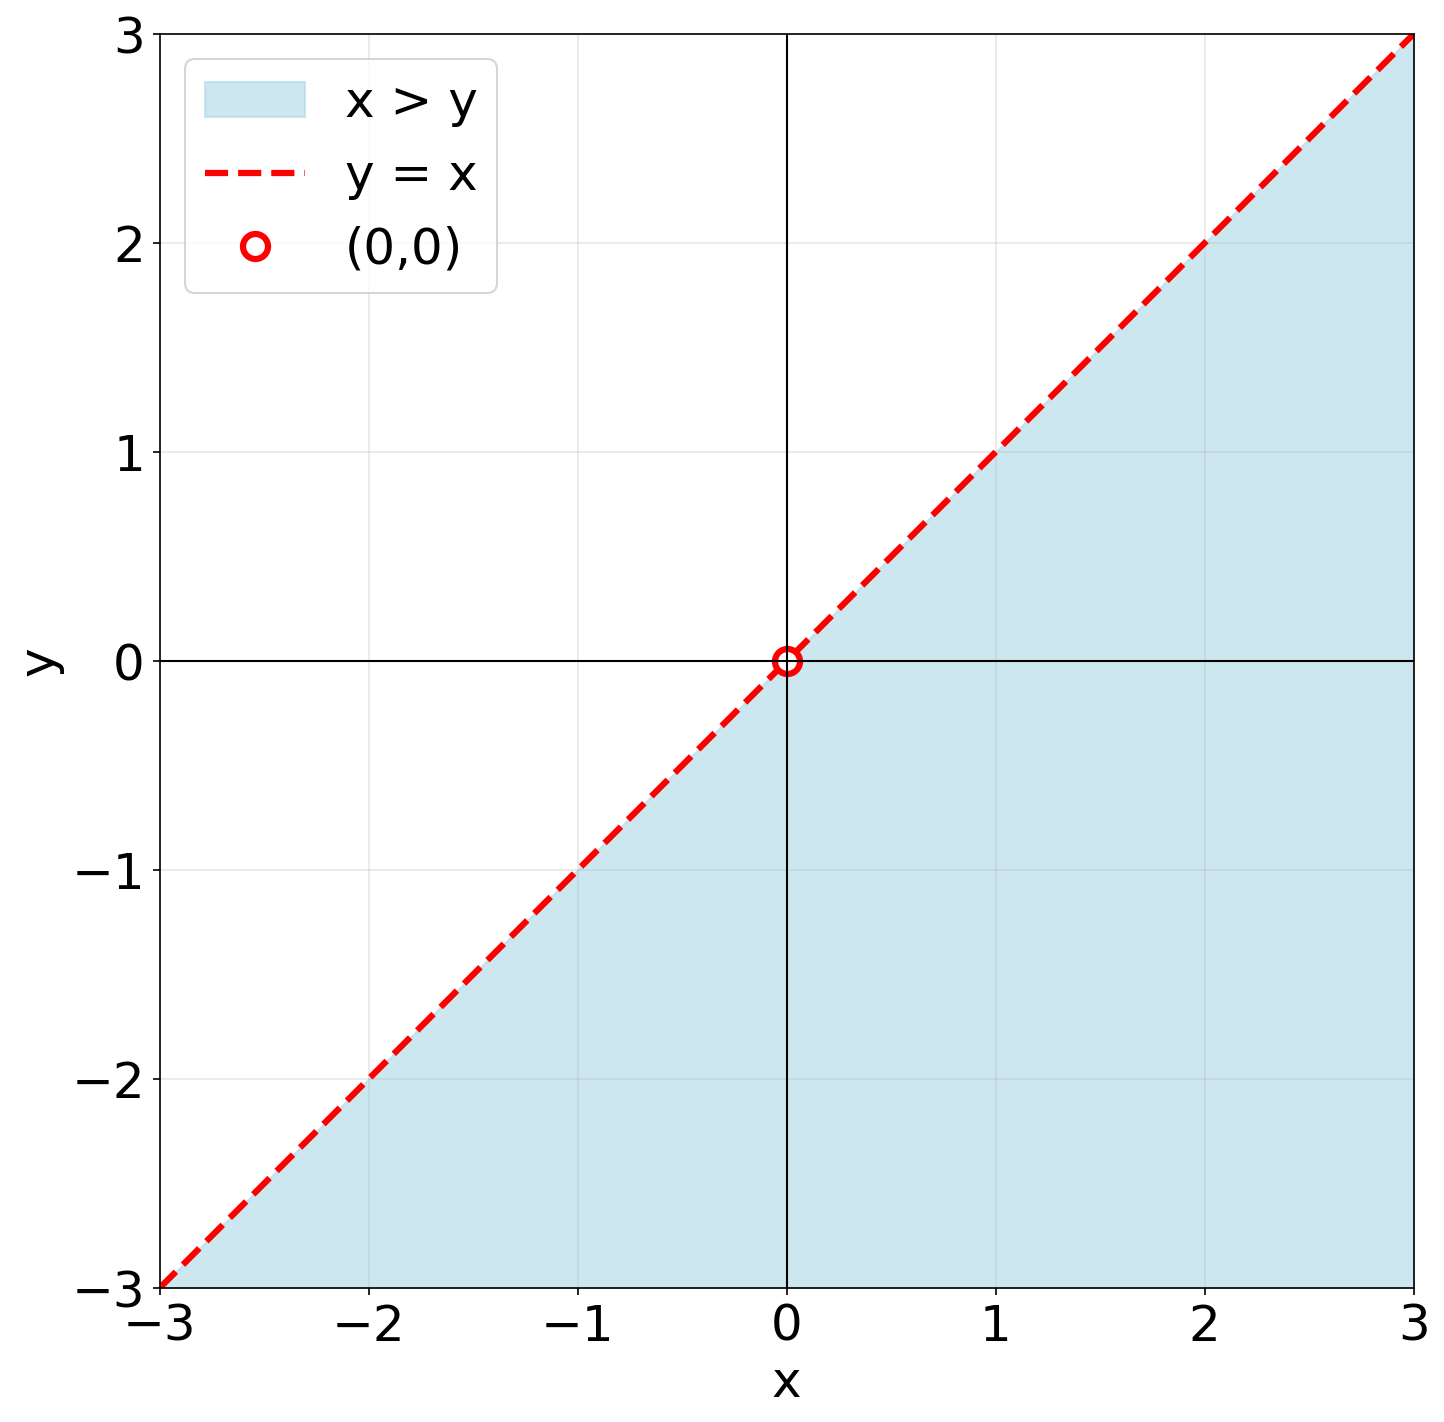
\includegraphics[width=0.52\textwidth]{res/graph1.png}
\end{figure}
